\section{Übereinstimmung Daten und Simulation}
\label{sec:aufgabe6}

Grundlage für Messungen neuer Physik ist immer eine sinnvolle Übereinstimmung
der Daten mit der Simulation, vor allem in einem Phasenraum, in dem der
Untergrund dominiert. Dafür werden zunächst die erwartete Anzahl der Events
berechnet, welche zu einer integierten Luminosität von
$\mathcal{L} = \SI{1}{\femto\barn}^{-1}$ korrespondieren. Mit Hilfe der Formel

\begin{equation}
N = \mathcal{L} \sigma A \epsilon
\label{eqn:erwartung}
\end{equation}

kann diese Anzahl berechnet werden. Dabei entspricht der Koeffizient
$\epsilon \cdot A$ den in Kapitel \ref{sec:aufgabe3}
berechneten Werten. Der Wirkungsquerschnitt der Prozesse ist zusammen mit
den erwarteten Events in Tabellle \ref{tab:Erwartungen} aufgelistet. Die erwarteten
Events sind für das ausgewählte Sample \texttt{data.mu.2.root} aufgelistet. Insgesamt
werden insgesamt $66.8647$ Untergrundevents erwartet. Gemessene Events nach der
Selektion in diesem Datenset sind $94$ Events.

\begin{table}[H]
    \centering
    \caption{Anzahl erwarteter Ereignisse für die einzelnen Prozesse im sample \texttt{data.mu.2.root}. Angegeben
    ist der zugehörige Wirkungsquerschnitt der für die Berechnung der einzelnen Werte nach Formel
    \eqref{eqn:erwartung} benötigt wird.}
    \label{tab:Erwartungen}
    \begin{tabular}{c|cc}
    \toprule
    Prozess & $\text{N}_\text{expected}$ & $\sigma$ / $\SI{}{\pico\barn}$ \\
    \midrule
    \texttt{ttbar}      &  3.0282   & 252.82    \\
    \texttt{singletop}  &  3.3576   & 52.47     \\
    \texttt{diboson}    &  2.9967   & 29.41     \\
    \texttt{wjets}      &  6.3202   & 2516.20   \\
    \texttt{zjets}      &  51.1618  & 36214     \\
    \texttt{zprime400}  &  103.4000 & 1.1e2     \\
    \texttt{zprime500}  &  77.0800  & 8.2e1     \\
    \texttt{zprime750}  &  18.8000  & 2.0e1     \\
    \texttt{zprime1000} &  51.7000  & 5.5       \\
    \texttt{zprime1250} &  17.8600  & 1.9       \\
    \texttt{zprime1500} &  7.8020   & 8.3e-1    \\
    \texttt{zprime1750} &  2.8200   & 3.0e-1    \\
    \texttt{zprime2000} &  1.3160   & 1.4e-1    \\
    \texttt{zprime2250} &  0.0630   & 6.7e-2    \\
    \texttt{zprime2500} &  0.0330   & 3.5e-2    \\
    \texttt{zprime3000} &  0.0113   & 1.2e-2    \\
    \bottomrule
    \end{tabular}
\end{table}

Die selektierten Events beziehen sich noch auf das gegebene Sample, mit individuellen
Wirkungsquerschnitten und Sample-Größen, je nach Prozess. Deswegen müssen noch
Gewichte eingeführt werden, die die MC-Samples auf das Datensample normieren. Diese
Gewichte werden mit Hilfe der Formel

\begin{equation}
w = \frac{\mathcal{L} \sigma}{\text{N}_\text{MC}}
\label{eqn:gewichte}
\end{equation}

berechnet. Dabei beschreibt $\text{N}_\text{MC}$ die Anzahl der MC events vor der
Vorselektion. Die Gewichte mit den Samplegrößen sind in Tabelle
\ref{tab:Gewichte} aufgelistet. Der Wirkungsquerschnitt ist in Tabelle
\ref{tab:Erwartungen} zu finden.

\begin{table}[H]
    \centering
    \caption{Berechnete Gewichte für die einzelnen Prozesse. Der für die Berechnung notwendige
    Wirkungsquerschnitt ist in Tabelle \ref{tab:Erwartungen} aufgelistet. Die integrierte
    Luminosität beträgt $\mathcal{L} = \SI{1}{\femto\barn}^{-1}$. Die Gewichte werden mit
    Hilfe von Formel \eqref{eqn:gewichte} berechnet.}
    \label{tab:Gewichte}
    \begin{tabular}{c|cc}
    \toprule
    Prozess & $\text{N}_\text{MC}$ & Gewichtung $w$ \\
    \midrule
    \texttt{ttbar}      & 7847944    & 0.03221     \\
    \texttt{singletop}  & 1468942    & 0.03572     \\
    \texttt{diboson}    & 922521     & 0.03188     \\
    \texttt{wjets}      & 66536222   & 0.54428     \\
    \texttt{zjets}      & 37422926   & 0.06724     \\
    \texttt{zprime400}  & 100000     & 1.10000     \\
    \texttt{zprime500}  & 100000     & 0.82000     \\
    \texttt{zprime750}  & 100000     & 0.20000     \\
    \texttt{zprime1000} & 100000     & 0.55000     \\
    \texttt{zprime1250} & 100000     & 0.19000     \\
    \texttt{zprime1500} & 100000     & 0.08300     \\
    \texttt{zprime1750} & 100000     & 0.03000     \\
    \texttt{zprime2000} & 100000     & 0.01400     \\
    \texttt{zprime2250} & 100000     & 0.00067     \\
    \texttt{zprime2500} & 100000     & 0.00035     \\
    \texttt{zprime3000} & 100000     & 0.00012     \\
    \bottomrule
    \end{tabular}
\end{table}

Diese Gewichte werden an die entsprechenden Samples mulipliziert. In sogenannten
Stacked Plots werden die einzelnen Untergrunde aufeinander gestapelt und
die Datenpunkte als overlay eingefügt um die Übereinstimmung von Daten und
Simulation zu Überprüfen. Exemplarisch werden in
Abbildung \ref{fig:stackedex} vier Stacked Plots auf
fehlerhafte Modellierung diskutiert, die restlichen werden im Anhang \ref{sec:stackedrest} aufgelistet.

\begin{figure}[H]
  \begin{subfigure}{0.5\textwidth}
    \centering
    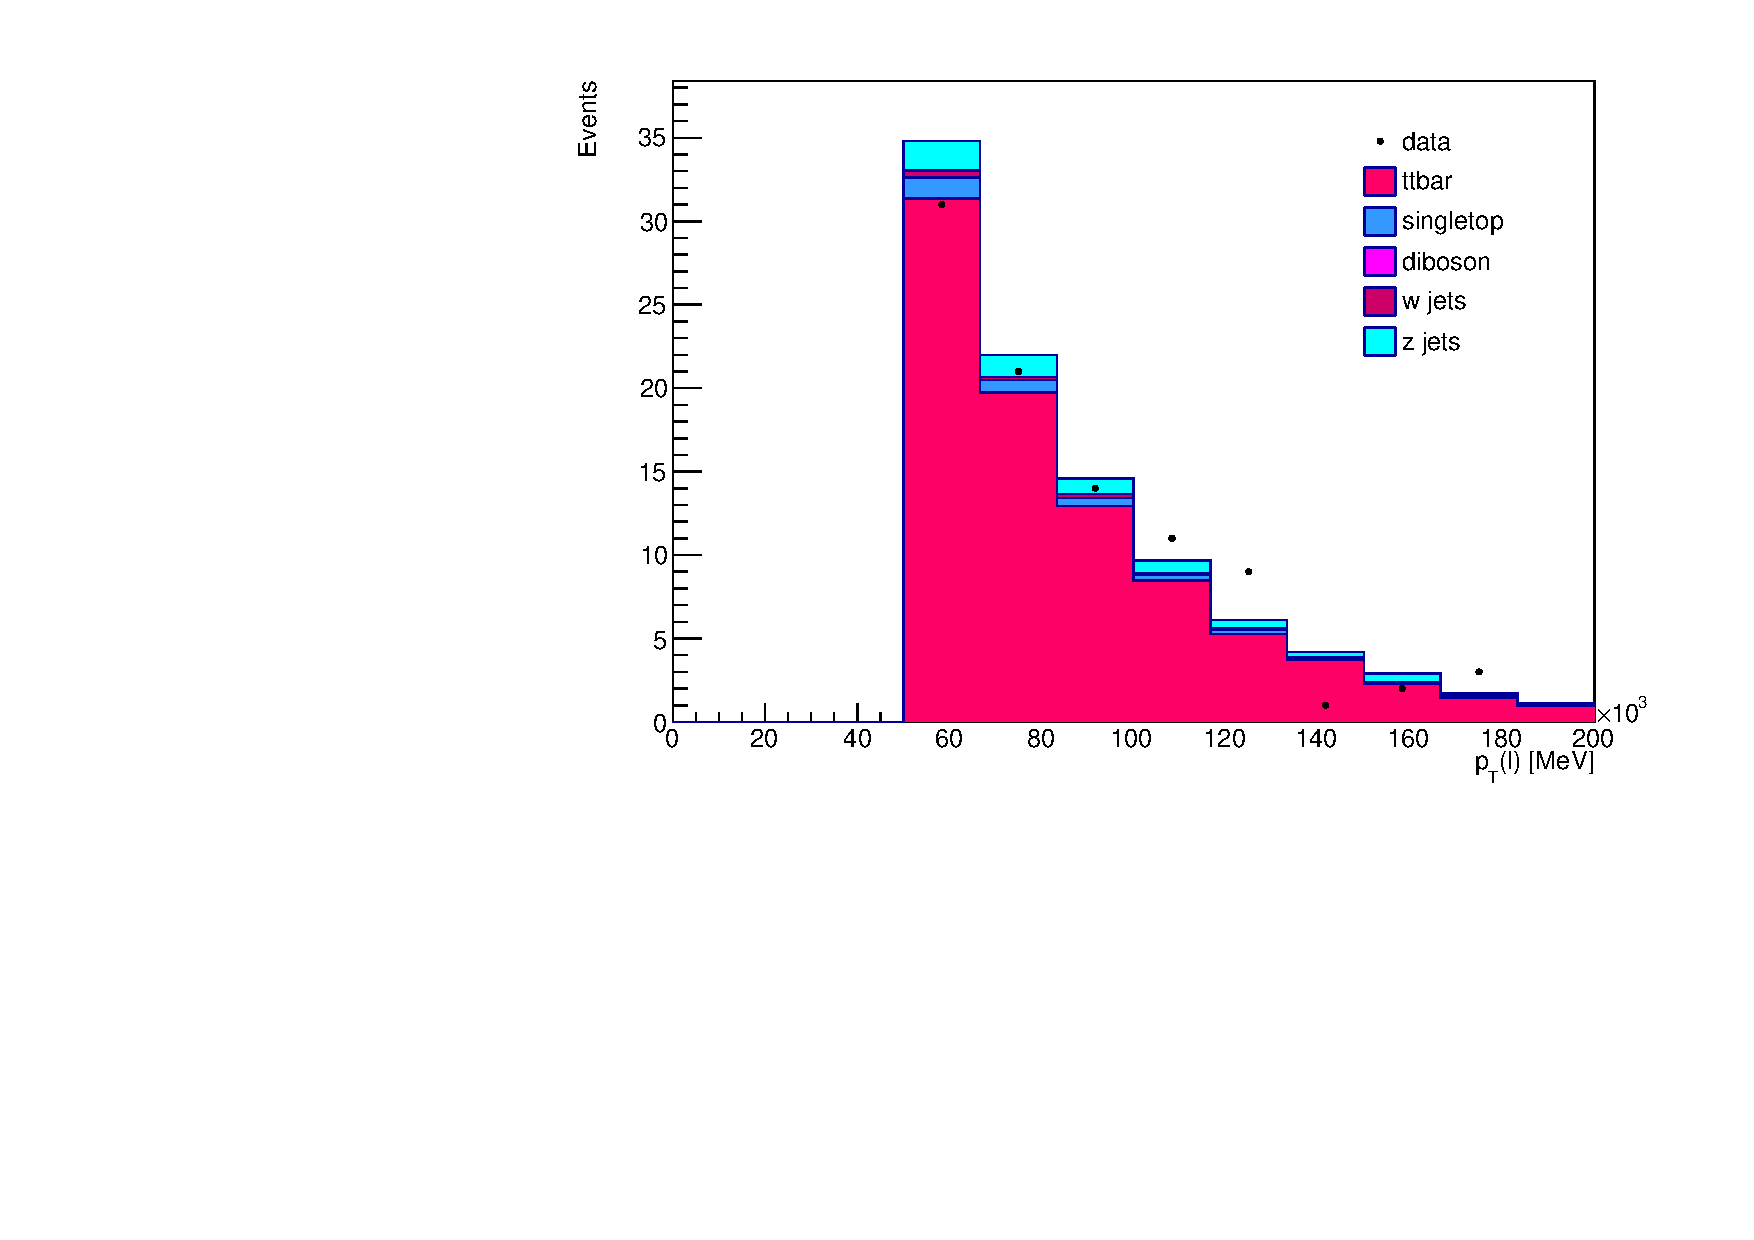
\includegraphics[width=\linewidth]{plots_and_txt/stacked_plots/stacked_lep_pt.pdf}
    \caption{}
    \label{fig:stacked_lep_pt}
  \end{subfigure}%
  \begin{subfigure}{0.5\textwidth}
    \centering
    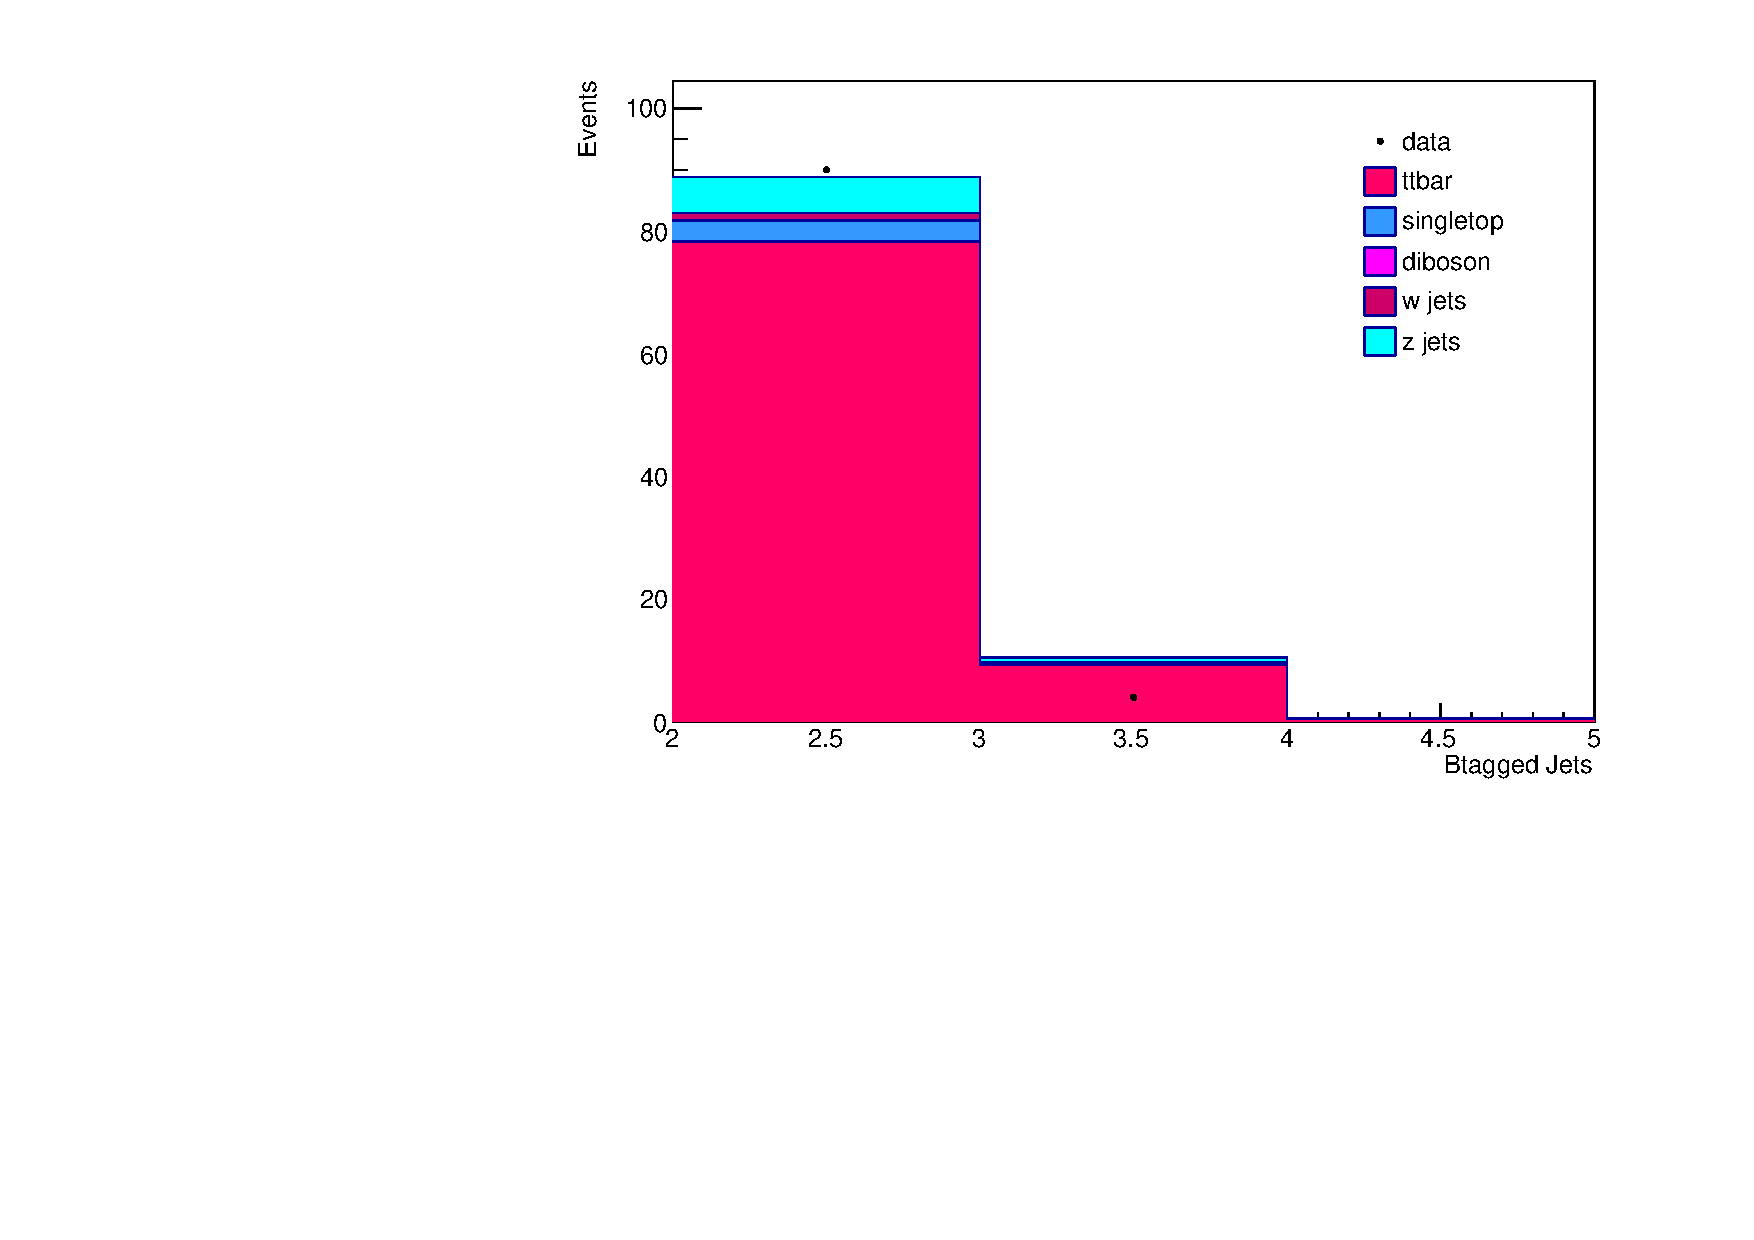
\includegraphics[width=\linewidth]{plots_and_txt/stacked_plots/stacked_btagged.pdf}
    \caption{}
    \label{fig:stacked_btagged}
  \end{subfigure}%
  \newline
  \begin{subfigure}{0.5\textwidth}
    \centering
    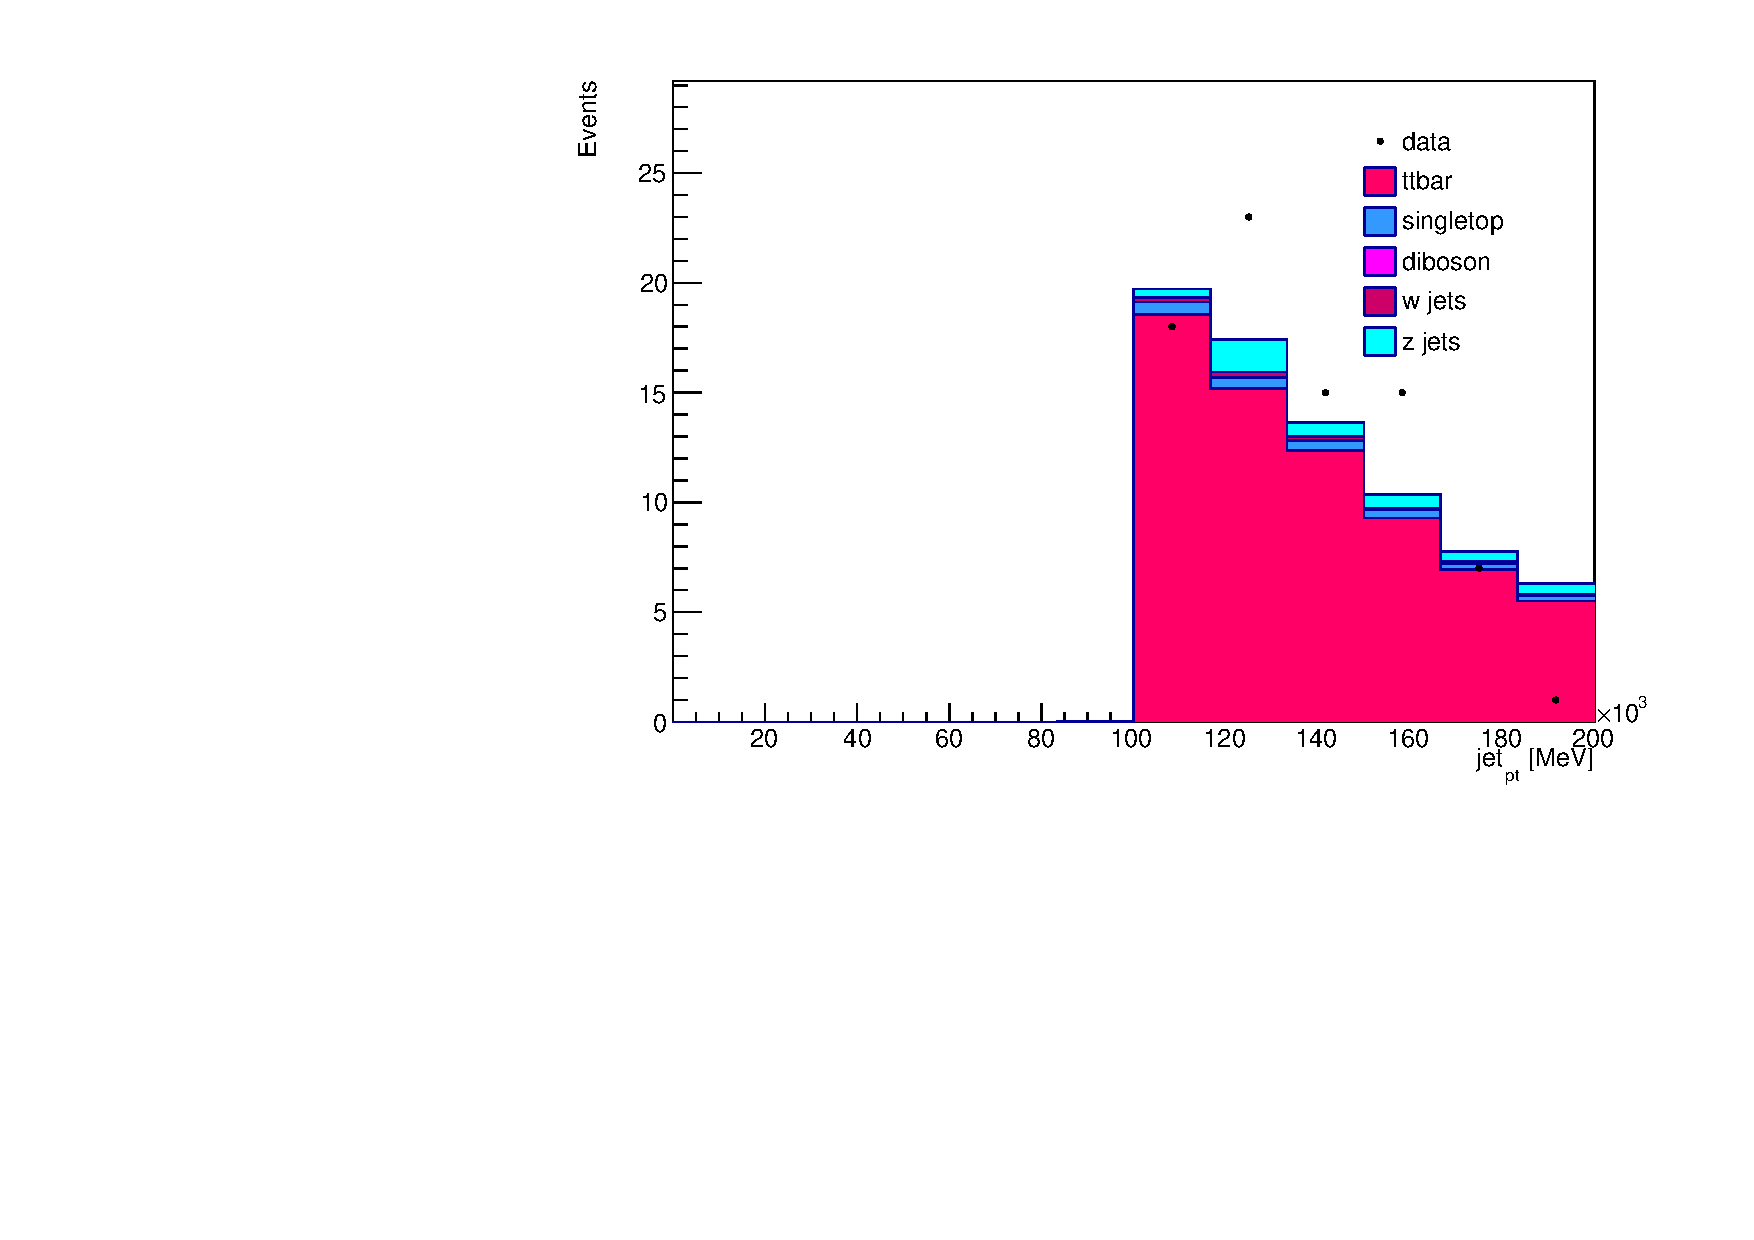
\includegraphics[width=\linewidth]{plots_and_txt/stacked_plots/stacked_jet_pt.pdf}
    \caption{}
    \label{fig:stacked_jet_pt_good}
  \end{subfigure}%
  \begin{subfigure}{0.5\textwidth}
    \centering
    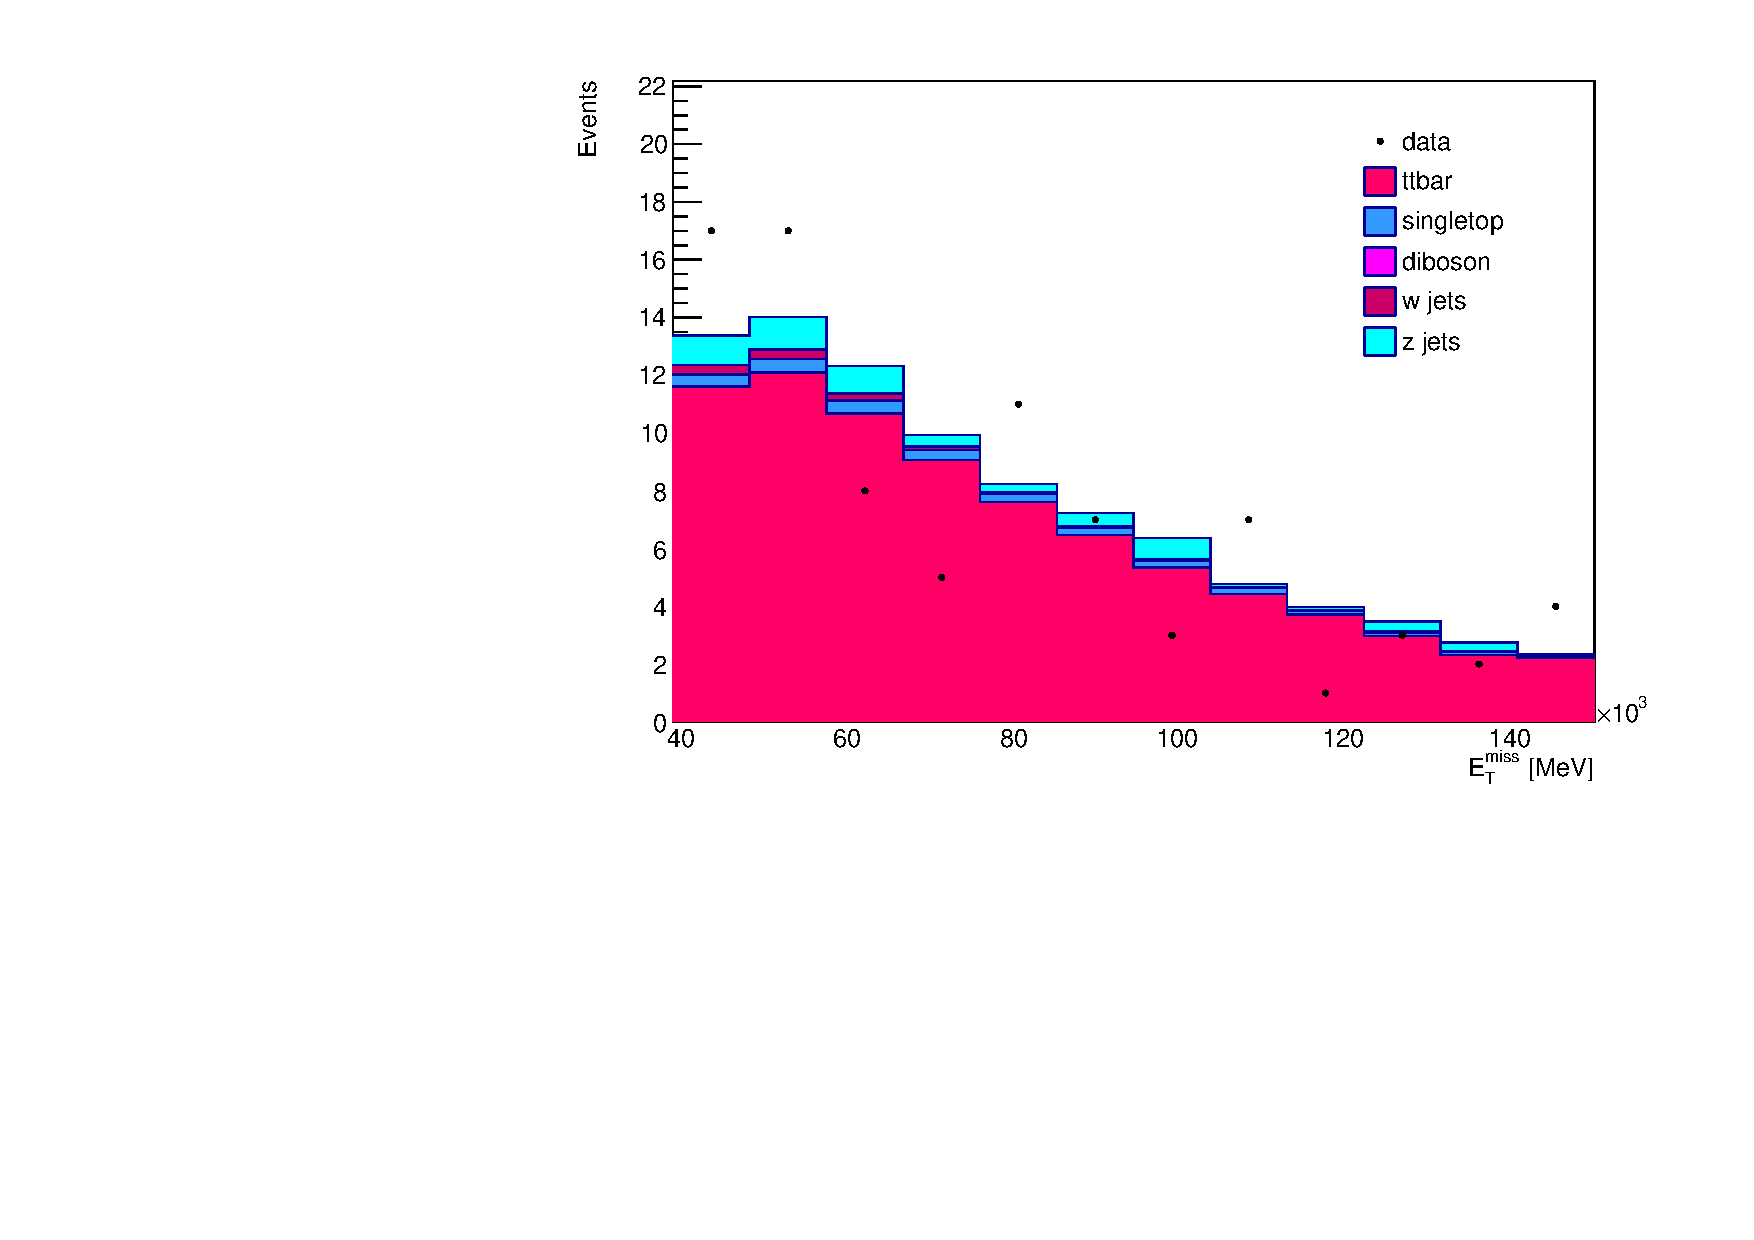
\includegraphics[width=\linewidth]{plots_and_txt/stacked_plots/stacked_met_et.pdf}
    \caption{}
    \label{fig:stacked_met_et}
  \end{subfigure}%
  \caption{Gestapelte Untergründe im Vergleich mit den selektierten Datensample.
  Zusehen sind der transverale Impuls der Myonen (\subref{fig:stacked_lep_pt}),
  die Anzahl an btagged Jets (\subref{fig:stacked_btagged}),
  der transverase Impuls des Jets mit dem höchsten transversalen Impuls des Events (\subref{fig:stacked_jet_pt_good}) und die fehlende transversal Energie (\subref{fig:stacked_met_et}).
  }
  \label{fig:stackedex}
\end{figure}


Die größte Diskrepanz ist in der Verteilung der fehlenden Transversalenergie
zu sehen. In den Bins, sind die Datenpunkte entweder deutlich über den
Untergrunddaten oder deutlich unter ihnen abgebildet. Ein erhöhter Datenpunkt könnte
prinzipiell einen Hinweis auf ein Signal liefern, da aber ebensoviele
Punkte deutlich unter dem Untergrundsignal sind, liegt der Ursprung vermutlich
eher in einem systematischen Fehler. Da diese Grafiken bereits deutlich
auf Monte Carlo Fehlmodellierungen hinweisen, verlieren die Ergebnisse
deutlich an Sigifikanz. \par

Als nächstes wird die Diskriminante untersucht.

\begin{figure}[H]
    \centering
    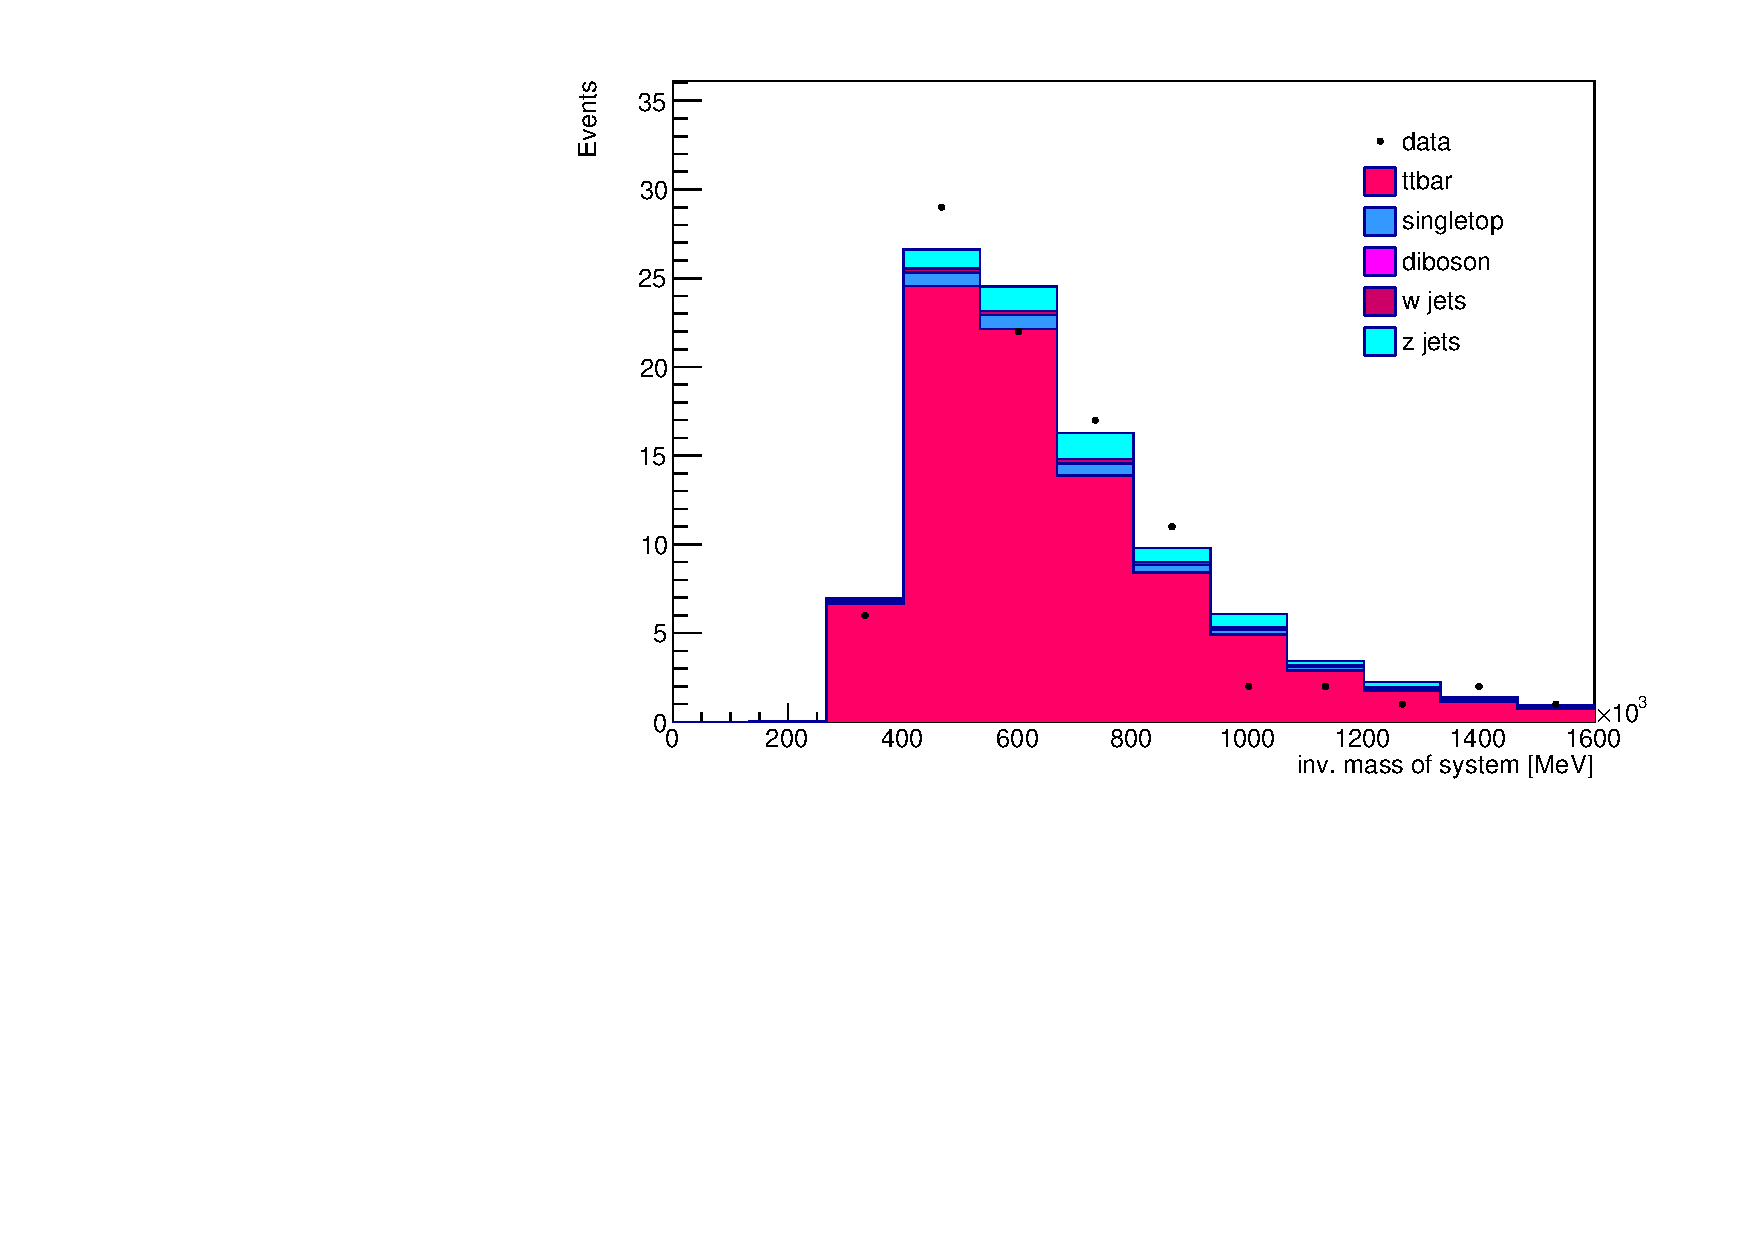
\includegraphics[width=\linewidth]{plots_and_txt/stacked_plots/stacked_disc.pdf}
    \caption{Verteilung der invarianten Masse des Systems, welches aus den vier Jets mit dem größten $p_T$, dem Lepton und dem Neutrino gebildet wird.}
    \label{fig:stacked_disc}
\end{figure}

Im zweiten und fünften Bin sind Exzesse der Daten über dem Untergrund feststellbar.
Jedoch auf Grund der vorher bemerkten Fehlmodellierung der Untergründe kann
hier nicht von einer Entdeckung oder einem Hinweis auf ein $Z^\prime$ Signal
gesprochen werden.
